\documentclass[conference]{IEEEtran}
\IEEEoverridecommandlockouts
% The preceding line is only needed to identify funding in the first footnote. If that is unneeded, please comment it out.
\usepackage{cite}
\usepackage{amsmath,amssymb,amsfonts}
%\usepackage{algorithmic}
\usepackage{graphicx}
\usepackage{float}
\usepackage{textcomp}
\usepackage{xcolor}
\def\BibTeX{{\rm B\kern-.05em{\sc i\kern-.025em b}\kern-.08em
    T\kern-.1667em\lower.7ex\hbox{E}\kern-.125emX}}

\usepackage{tikz}
\usepackage{pgfplots}

\usepackage{algorithm}
\usepackage[noend]{algpseudocode}
\makeatletter
\renewcommand{\ALG@beginalgorithmic}{\footnotesize}
\makeatother

\algnewcommand\algorithmicswitch{\textbf{switch}}
\algnewcommand\algorithmiccase{\textbf{case}}
\algnewcommand\algorithmicotherwise{\textbf{otherwise}}

\algdef{SE}[SWITCH]{Switch}{EndSwitch}[1]{\algorithmicswitch\ #1\ \algorithmicdo}{\algorithmicend\ \algorithmicswitch}%
\algdef{SE}[CASE]{Case}{EndCase}[1]{\algorithmiccase\ #1}{\algorithmicend\ \algorithmiccase}%
\algdef{SE}[OTHERWISE]{Otherwise}{EndOtherwise}[1]{\algorithmicotherwise\ #1}{\algorithmicend\ \algorithmicotherwise}%
\algtext*{EndSwitch}%
\algtext*{EndCase}%
\algtext*{EndOtherwise}%

\usepackage[bahasa]{babel}

\begin{document}

\title{DESAIN DAN IMPLEMENTASI APLIKASI PENGOLAHAN SKYLINE QUERY PADA UNCERTAIN DATA STREAMING OLEH TITIK BERGERAK DAN OBJEK TIDAK BERGERAK PADA JARINGAN JALAN RAYA}

\author{Syukron Rifai'il Muttaqi, Royyana Muslim Ijtihadie, dan Bagus Jati Santoso\\
Departemen Informatika, Fakultas Teknologi Informasi dan Komunikasi, Institut Teknologi Sepuluh Nopember (ITS)\\
Jl. Arief Rahman Hakim, Surabaya 60111 Indonesia\\
\textit{e-mail}: syukronrifai@gmail.com\textsuperscript{1)}, roy@if.its.ac.id\textsuperscript{2)}, bagus@if.its.ac.id\textsuperscript{3)}
}

\maketitle

\renewcommand\abstractname{\textit{Abstrak}}
\renewcommand\IEEEkeywordsname{Kata kunci}

\begin{abstract}
Semakin banyaknya pengguna teknologi mendorong proses pencarian data semakin cepat. Diantara permasalahan mengenai pemrosesan data yaitu pencarian objek terbaik pada data spasial. Pemrosesan data pada jaringan jalan raya menjadi berbeda jika lokasi titik \textit{query} yang berpindah-pindah. Dalam beberapa kasus, data objek berupa \textit{uncertain data} dan bersifat \textit{streaming}.

Artikel ini mengusulkan algoritme \textit{Continuous Streaming $ \mathbf{d_\varepsilon} $-distance Skyline Query}, sebuah algoritme untuk memproses \textit{Skyline Query} pada jaringan jalan raya dengan \textit{uncertain data streaming}. Algoritma ini menggunakan $ \mathbf{d_\varepsilon} $ sebagai jarak maksimal objek dapat menjadi objek terbaik dari titik \textit{query}. Hasil uji coba menunjukkan bahwa metode yang diusulkan memiliki waktu komputasi 600 kali lebih cepat dan penggunaan memori lebih hemat 1500 kali dibandingkan metode \textit{naive}.
\end{abstract}



\begin{IEEEkeywords}
\textit{skyline query}, \textit{uncertain data streaming}, jaringan jalan raya
\end{IEEEkeywords}

\section{Pendahuluan}
Cepatnya pertumbuhan dan perkembangan teknologi memicu banyaknya data yang diproduksi. Banyaknya data yang berpindah mendorong proses pengolahan data menjadi lebih cepat. Bertambahnya pengguna teknologi dan internet juga mendorong frekuensi pengambilan data agar menjadi lebih efektif dan efisien.

Pada kasus tertentu, pengguna teknologi membutuhkan pengambilan dan pemrosesan data terbaik dengan cepat dan tepat. Diantara permasalahan mengenai pemrosesan data yaitu pencarian objek yang paling unggul pada data spasial. Jaringan jalan raya \textit{road network} adalah salah satu bentuk data yang bersifat spasial. Pencarian data pada jaringan jalan raya bersifat relatif terhadap titik \textit{query} tertentu. Jika titik berpindah, maka perlu pemrosesan ulang data yang unggul sesuai titik terakhir. Metode ini kurang efisien karena biaya komputasi sangat tergantung pada titik \textit{query}. Jika titik \textit{query} selalu berpindah, maka dibutuhkan pemrosesan tersendiri yang bersifat kontinu sehingga tidak diperlukan banyak komputasi ketika titik \textit{query} mengalami perpindahan.

Banyaknya teknologi yang digunakan sekarang membuat \textit{uncertain data} semakin banyak. \textit{Query} data terunggul dari \textit{uncertain data} memerlukan metode tersendiri untuk menyelesaikannya.
	
Diantara algoritme pencarian data paling unggul adalah metode \textit{skyline}, termasuk pada jaringan jalan raya. Metode ini dapat diterapkan pada jaringan jalan raya dengan menggunakan \textit{uncertain data}. Struktur data khusus diperlukan agar proses pencarian data/\textit{query} dapat dilakukan secara \textit{real time}.

Artikel ini membahas mengenai metode pencarian objek yang menjadi \textit{skyline} pada jaringan jalan raya. Masing-masing objek berupa \textit{uncertain} data dan bersifat streaming.

\section{Tinjauan Pustaka}
\subsection{Skyline}
Pada himpunan titik pada multidimensi $ d $, \textit{skyline} dari data tersebut adalah titik yang tidak didominasi oleh titik lain. Titik $ o $ mendominasi titik $ o' $, dinotasikan sebagai $ o \prec o' $, apabila setiap nilai dari atribut pada $ o $ lebih baik atau sama dengan yang terdapat pada $ o' $ dan setidaknya terdapat satu atribut $ o $ yang lebih baik daripada yang terdapat pada $ o' $. Titik titik yang mendominasi tersebut disebut dengan \textit{skyline points} $ (SP) $.

\begin{figure}[!htb]
	\centering
	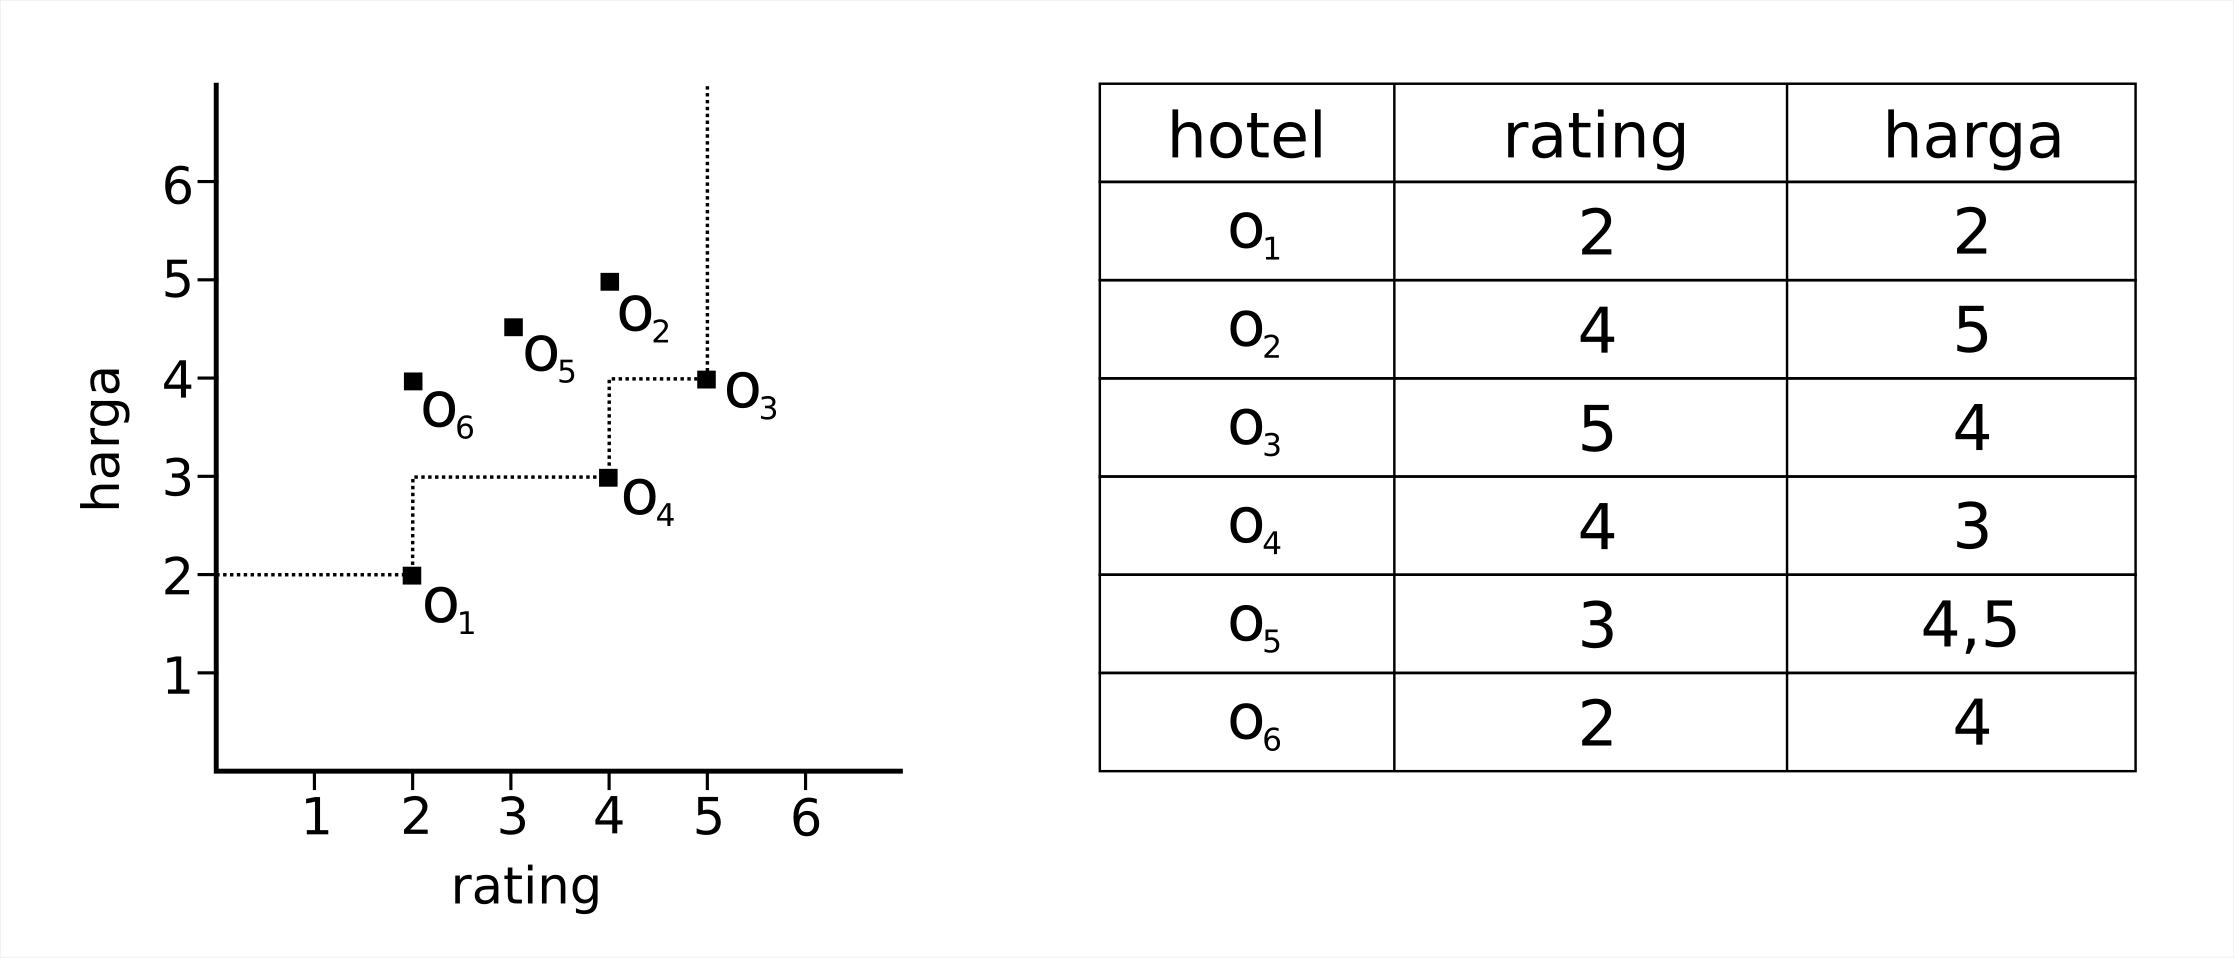
\includegraphics[width=8cm]{imgs/skyline.png}
	\caption{Contoh \textit{skyline} sederhana}
	\label{fig:skyline-traditional}
\end{figure}

%%Sebagai contoh, seseorang ingin mencari hotel terbaik dari sekumpulan hotel. Sebuah hotel dikatakan lebih baik apabila memiliki rating yang lebih tinggi dan/atau harga yang lebih rendah. \textit{SP} pada Gambar \ref{fig:skyline-traditional} adalah hotel yang memiliki ranking yang tinggi dan harga yang rendah. Objek yang menjadi bagian dari \textit{SP} dari adalah hotel $ o_1 $, $ o_3 $ dan $ o_4 $. Ketiga objek tersebut tidak didominasi oleh objek yang lain. Hotel $ o_6 $ didominasi oleh $ o_4 $ pada atribut rating dan harga, didominasi oleh $ o_1 $ pada atribut harga, dan didominasi oleh $ o_3 $ pada atribut rating. Demikian juga untuk objek $ o_2 $ dan $ o_6 $, masing-masing didominasi oleh objek lain. Dengan demikian, hanya $ o_1 $, $ o_3 $, dan $ o_4 $ yang tidak didominasi objek lain\cite{continuousdbased}.

\subsection{\textit{Skyline Query} pada Jaringan Jalan Raya}
\textit{Skyline query} tradisional seperti pada Gambar \ref{fig:skyline-traditional} hanya menggunakan atribut statis sebagai penentuan \textit{SP}, yaitu atribut ranking dan hotel. Jika \textit{skyline query} ditempatkan pada jaringan jalan raya seperti pada Gambar 2.3, maka perlu menambahkan jarak sebagai salah satu atribut dalam menentukan \textit{SP}.

Pada Gambar \ref{fig:skyline-traditional}, hotel yang menjadi \textit{SP} adalah $ o_1 $, $ o_2 $ dan $ o_3 $. Ketika hotel $ o_1 $ hingga $ o_5 $ dimasukkan dalam jaringan jalan raya seperti pada Gambar \ref{fig:skyline-road}, $ o_5 $ tidak lagi didominasi oleh $ o_4 $ sehingga $ o_5 $ bergabung menjadi bagian dari \textit{SP}. Hal tersebut dikarenakana jarak antara titik \textit{query} $ q $ dengan $ o_5 $ tidak didominasi oleh $ o_1 $, $ o_2 $ maupun $ o_3 $. Atribut jarak ini akan berubah-ubah sesuai dengan jarak titik \textit{query} $ q $ dengan masing-masing objek. Oleh karena itu, atribut jarak disebut sebagai atribut dinamis \cite{continuousdbased}.

Skyline \textit{query} yang hanya menggunakan atribut statis dapat dicari \textit{SP}-nya dengan sekali proses \textit{query}, atau disebut dengan \textit{snapshot skyline query}. Pada kasus jaringan jalan raya, titik \textit{query} dapat bergerak dengan leluasa. Metode naif yang paling mudah diimplementasikan yaitu melakukan proses \textit{query} ketika titik \textit{query} bergerak. Namun hal ini tentunya sangat tidak efektif mengingat banyaknya komputasi yang dilakukan apabila terdapat banyak titik \textit{query} dan titik \textit{query} tersebut sering bergerak.

Pada kasus tertentu objek \textit{SP} memiliki jarak yang sangat jauh dari titik \textit{query}. Objek tersebut seringkali tidak diinginkan karena kita mencari titik \textit{query} yang dekat karena untuk mencapai objek yang jauh membutuhkan biaya lebih besar dalam hal transportasi.

Y.-K. Huang et al. telah mengusulkan metode untuk menyelesaikan permasalahan ini dengan metode \textit{continuous $ d_\varepsilon $-skyline query} ($ Cd_\varepsilon-SQ $) \cite{continuousdbased}. Metode ini menggunakan jarak $ d_\varepsilon $ sebagai batas maksimal jarak antara titik \textit{query} dengan objek.

$ Cd_\varepsilon-SQ$ didefinisikan sebagai: Diketahui jalan $ P_q $ sebagai jalan tempat titik \textit{query} $ q $ bergerak diatasnya, himpunan objek $ S_o $, dan jarak $ d_\varepsilon $. Kueri $ Cd_\varepsilon-SQ $ menghasilkan himpunan skyline point, $ SP_p $ pada setiap titik $ p $ pada $ P_q $, yang memiliki jarak antara $ o \in SP_p $ ke titik p kurang dari sama dengan $ d_\varepsilon $. $ SP $ yang memenuhi $ Cd_\varepsilon-SQ $ dinotasikan sebagai $ d_\varepsilon-SP $.

\begin{figure}[H]
	\centering
	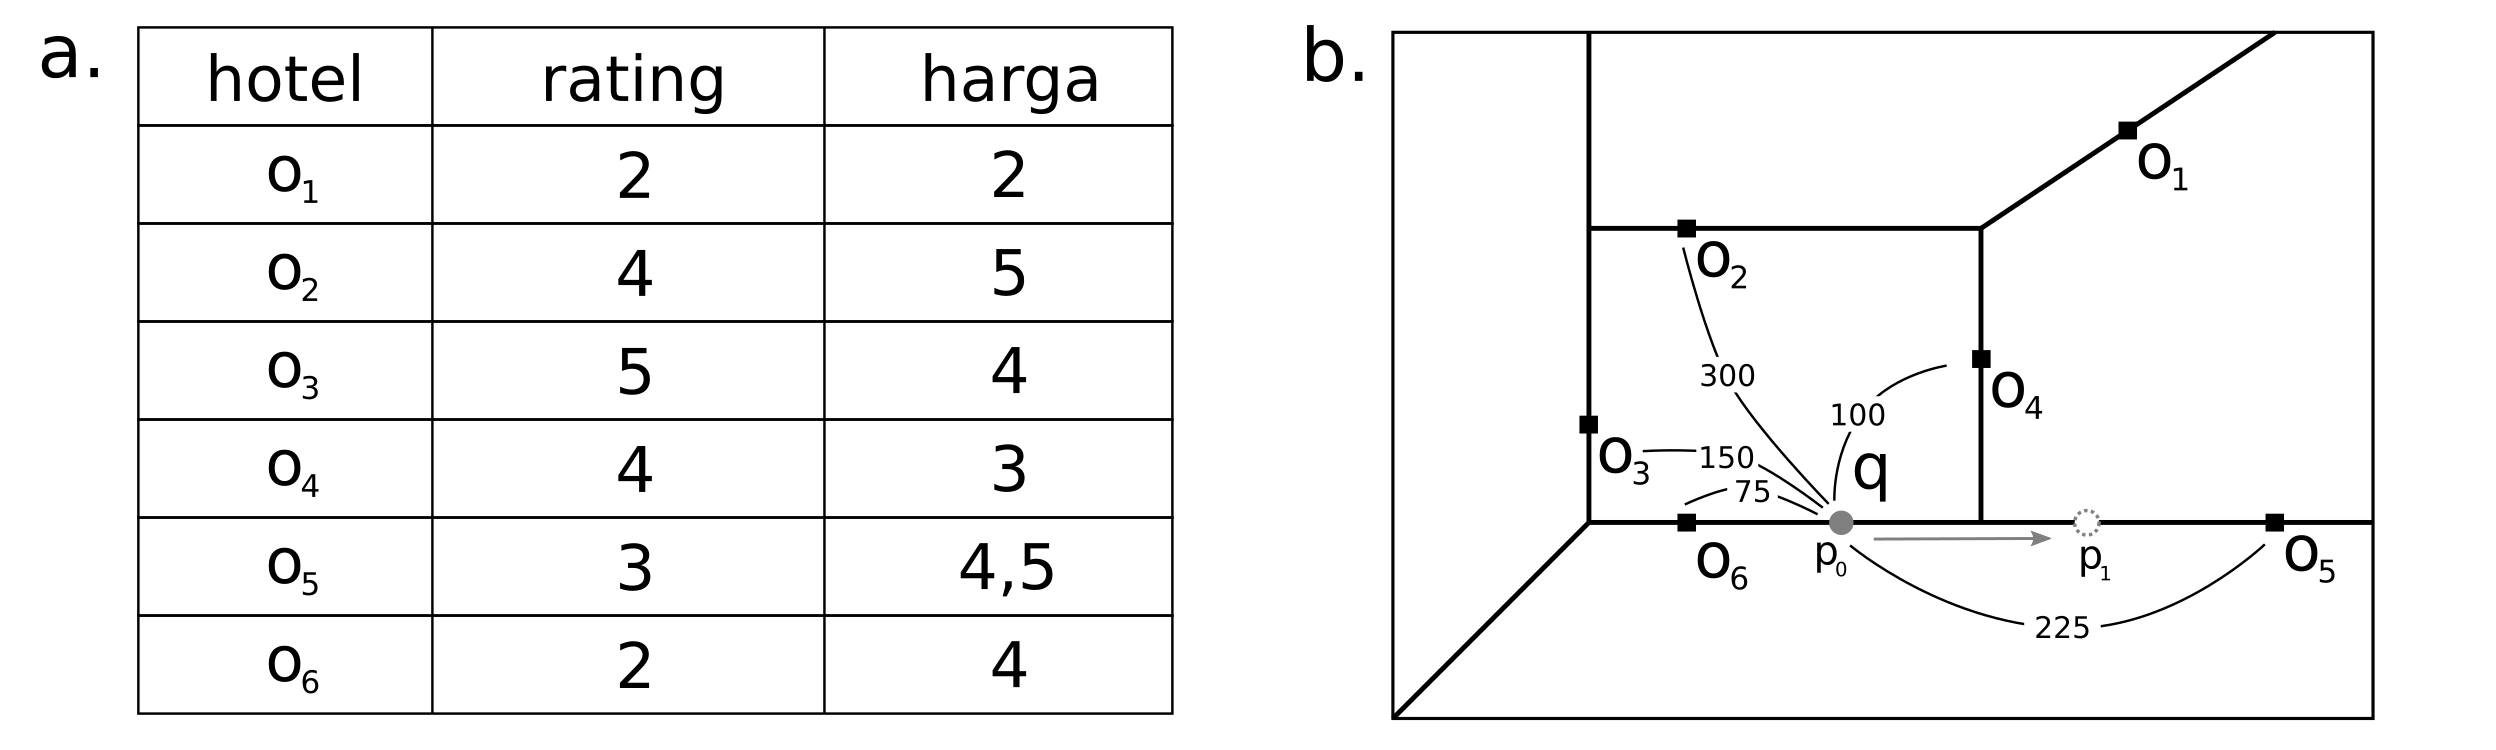
\includegraphics[width=9cm]{imgs/skylineroad-new.png}
	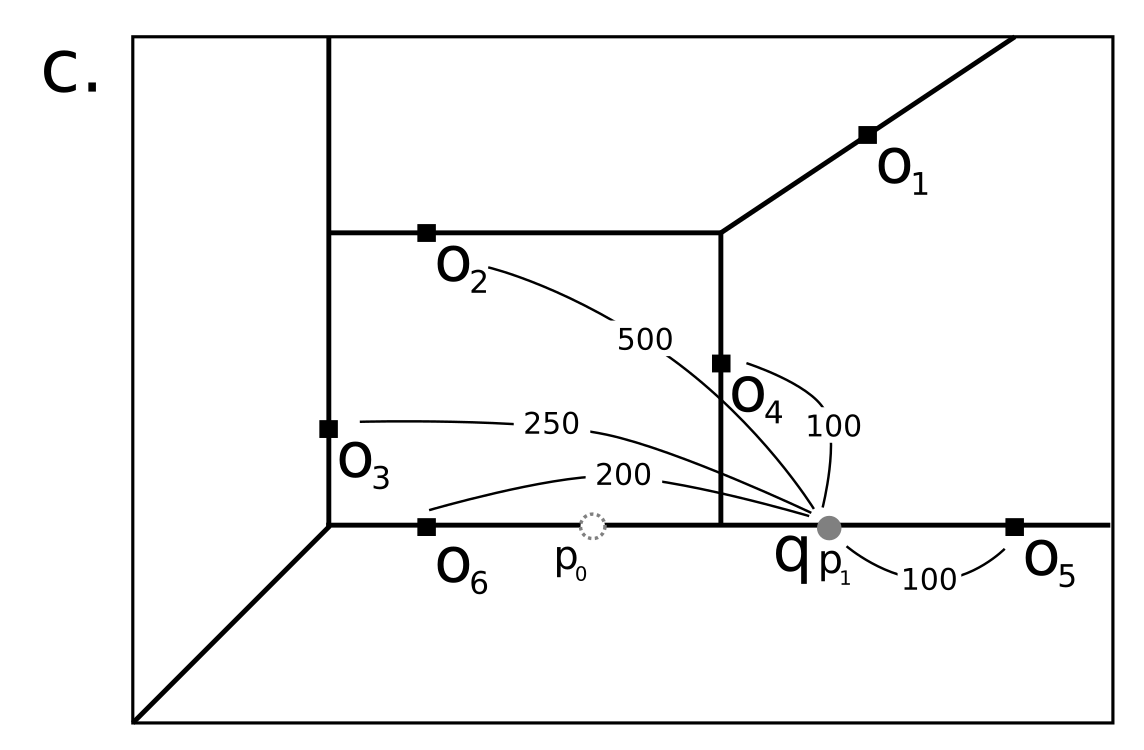
\includegraphics[width=5cm]{imgs/skylineroad-new-2.png}
	\caption{Contoh \textit{skyline} pada jaringan jalan raya}
	\label{fig:skyline-road}
\end{figure}

Gambar \ref{fig:skyline-road} mengilustrasikan pemrosesan \textit{skyline} pada jaringan jalan raya. Gambar \ref{fig:skyline-road}(a) menampilkan atribut statis dari keempat objek. Contoh tersebut mensimulasikan pencarian $ d_\varepsilon-SP $ pada titik \textit{query} \textit{q} yang bergerak dari titik $ p_1 $ ke $ p_2 $. Ketika \textit{q} berada pada koordinat $ p_1 $(lihat Gambar \ref{fig:skyline-road}(b)), anggota dari $ d_\varepsilon-SP $ hanyalah $ o_2 $. $ o_4 $ tidak dapat menjadi $ d_\varepsilon-SP $ karena didominasi oleh $ o_2 $ dalam hal atribut statis(harga dan rating) maupun dinamis(jarak). $ o_1 $ dan $ o_3 $ tidak tergabung dalam $ d_\varepsilon-SP $ karena memiliki jarak lebih dari $ d_\varepsilon $. Selanjutnya, seperti yang terlihat pada Gambar \ref{fig:skyline-road}(c), titik \textit{query} $ q $ bergerak ke kiri sampai tepat di titik $ p_2 $ sehingga jarak antara titik \textit{query} $ q $ dengan $ o_2 $ dan $ o_4 $ menjadi sama. Ketika titik \textit{query} $ q $ bergerak ke kiri, $ o_4 $ menjadi lebih dekat kepada $ q $ dibandingkan $ o_2 $. Dengan demikian, $ o_2 $ tergabung menjadi $ d_\varepsilon-SP $ karena jarak $ o_2 $ tidak lagi didominasi oleh $ o_4 $. Selanjutnya $ d_\varepsilon-SP $-nya adalah $ o_2 $ dan $ o_4 $.

Dalam menentukan $ d_\varepsilon-SP $, yang pertama dilakukan adalah menghitung jarak terdekat antar dua objek. Penghitungan tersebut dapat dilakukan dengan algoritme Djikstra atau A*. Perlu digarisbawahi, penghitungan jarak terdekat membutuhkan sumber daya yang besar apabila terdapat banyak jalan(\textit{edge}) dan persimpangan(\textit{node}). Diantara hal yang menjadi tantangan adalah titik \textit{query} seringkali berpindah-pindah sehingga diperlukan metode khusus agar komputasi tidak dilakukan berulang kali dan menggunakan sumber daya yang banyak \cite{continuousdbased}.

\subsection{\textit{Uncertain Data}}
Pemrosesan  \textit{uncertain data} mendapat banyak perhatian pada beberapa tahun terakhir. \textit{Uncertain data} dapat ditemukan pada berbagai bidang, seperti jaringan sensor, jaringan RFID, sistem pelacakan lokasi menggunakan GPS, dan sosial media \cite{surveyuncertaindata}. Beberapa perangkat memang menghasilkan data yang cenderung tidak pasti (\textit{uncertain}). Sebagai contoh, data yang dihasilkan oleh sensor cenderung tidak pasti karena hilangnya data ketika transmisi, galat pada perangkat sensor itu sendiri atau karena lingkungan yang berubah-ubah \cite{effectiveprob}.

Seringkali data pada lingkungan bersifat dinamis dan kontinu. Sebagai contoh, pada jaringan sensor, \textit{gateway sensor} mengirim hasil secara kontinu, pemantauan cuaca mendapatkan data secara kontinu dengan komputasi waktu nyata. Hal tersebut menjadi tantangan tersendiri, yaitu pemrosesan \textit{uncertain data streaming} dengan efektif dan efisien sehingga hasil didapatkan di waktu itu juga \cite{effectiveprob}.

\section{Metode}
Bab ini memaparkan mengenai struktur data grid indeks serta algoritma yang digunakan pada struktur data tersebut.

\begin{table}[htbp]
	\caption{Ringkasan notasi}
	\begin{center}
		\begin{tabular}{| p{2cm} | p{5cm} |}
		\hline
		\textbf{Simbol} & \textbf{Deskripsi} \\ \hline
		$ d $ & Dimensi data \\ \hline
		$ x[i] $ & Nilai dari \textit{tuple} $ x $ pada dimensi ke-$ i $  \\ \hline
		$ X $ & Objek \textit{uncertain data}, $ x \in X $ \\ \hline
		$ U $ & \textit{Uncertain data streaming}, $ X \in U $ \\ \hline
		$ Y \prec x $ & Objek $ Y $ mendominasi \textit{instance} $ x $ \\ \hline
		$ X \prec Y $ & Objek $ X $ mendominasi objek $ Y $ \\ \hline
		$ SP $ & \textit{Skyline Point}, himpunan objek yang menjadi \textit{skyline} \\ \hline
		$ Pr(x) $ & Probabilitas tuple $ x $ \\ \hline
		$ SkyPr(x) $ & Probabilitas kejadian $ x $ menjadi anggota dari \textit{skyline} \\ \hline
		$ L $ & \textit{Landmark} \\
		\hline
		\end{tabular}
		\label{tab:istilah-bab3}
	\end{center}
\end{table}

\subsection{Struktur Data}
Jaringan jalan raya menggunakan jalan dan persimpangan sebagai objek utamanya. Hal tersebut dapat tersebut dapat dimodelkan dengan \textit{undirected weighted graph} yang terdiri dari \textit{node} dan \textit{edge}. \textit{Node} sebagai persimpangan dan \textit{edge} sebagai jalan. Struktur ini efisien untuk pencarian data pada peta.

Struktur graf sederhana menjadi sangat berat untuk diolah apabila terdapat terlalu banyak \textit{node}, \textit{edge}, dan objek di dalamnya. Penulis menggunakan struktur data grid indeks pemrosesan data. \textbf{Grid indeks} adalah struktur graf yang terbagi-bagi menjadi kotak-kotak dengan ukuran $ N \times N $. Setiap \textit{edge} dan \textit{node} menempati grid pada indeks $ m $ dan $ n $.

Struktur grid menampung tiga tabel, yaitu tabel objek, \textit{node}, dan \textit{edge}. Perhatikan tabel objek pada Tabel \ref{tab:objek}, setiap objek koordinat $ x $, $ y $, dan \textit{instances}. Atribut \textit{instances} berisi \textit{tuple-tuple} kejadian/titik dari objek. Dalam model matematis, setiap objek \textit{X} memiliki \textit{tuple-tuple} \textit{x}, $ x \in X $. Setiap tuple memiliki probabilitas yang dinotasikan dengan $ Pr(x) $. Jumlah probabilitas pada semua \textit{tuple} adalah 1, artinya $ \sum_{x \in X} Pr(x) = 1 $. Sebagai contoh, beberapa \textit{instance} di satu objek pada bidang 2 dimensi dapat ditulis dengan $ [(4, 5, 0.1), (5, 6, 0.5), (5, 7, 0.4)] $.

\begin{table}[htbp]
	\caption{Objek}
	\begin{center}
		\begin{tabular}{| p{2cm} | p{5cm} |}
			\hline
			\textbf{Atribut} & \textbf{Deskripsi} \\ \hline
			$ id $ & ID \textit{objek} \\ \hline
			$ x $ & Koordinat X \\ \hline
			$ y $ & Koordinat Y \\ \hline
			$ e $ & Edge tempat objek berada \\ \hline
			$ instances $ & Semua instance dari objek \\
			\hline
		\end{tabular}
		\label{tab:objek}
	\end{center}
\end{table}

\begin{figure}[H]
	\centering
	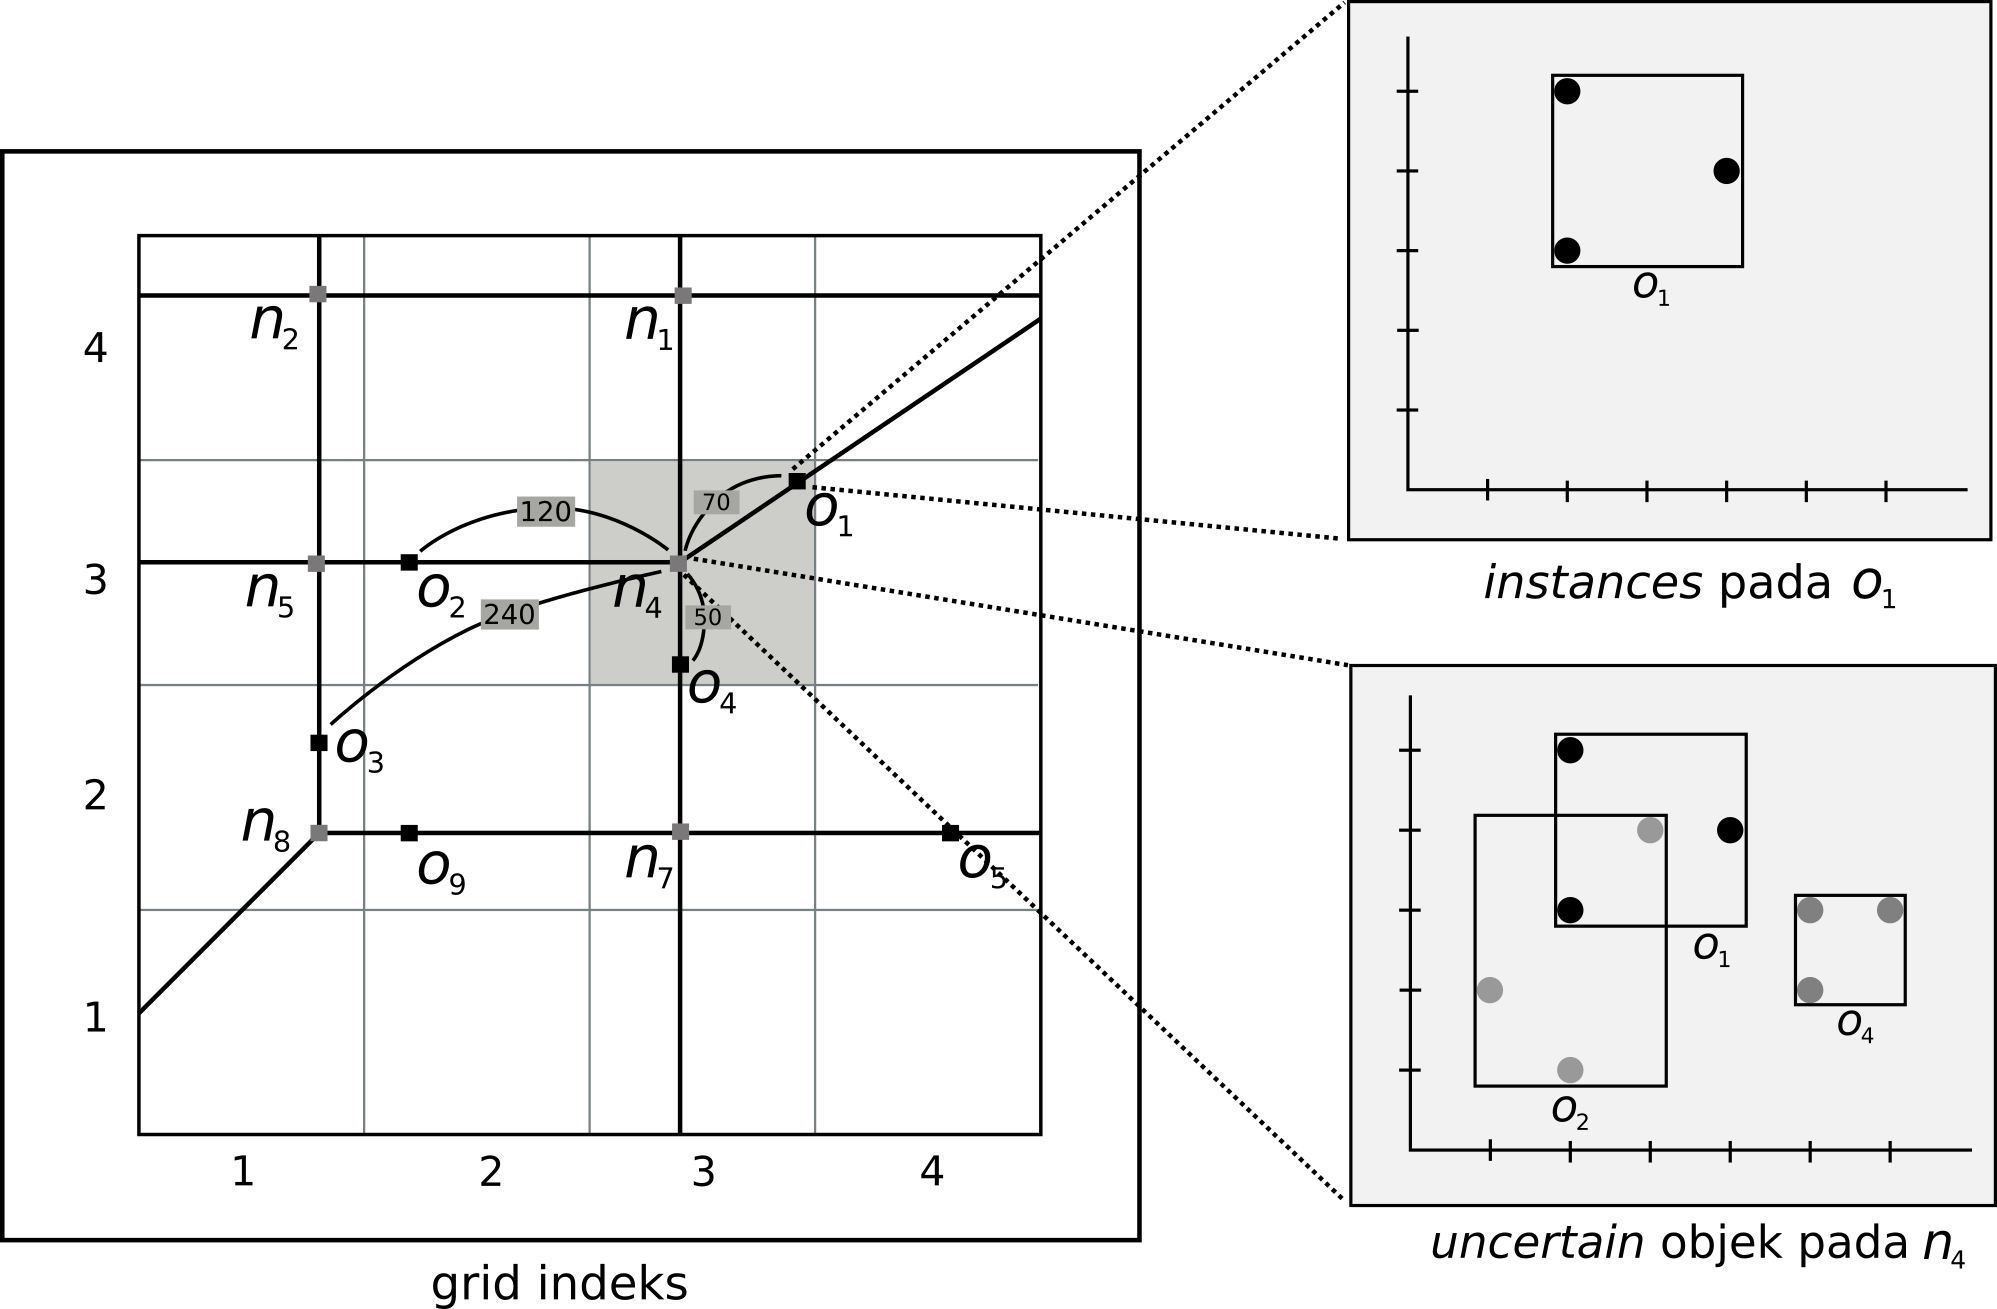
\includegraphics[width=9cm]{imgs/struktur-data.png}
	\caption{Struktur data grid indeks}
	\label{fig:grid}
\end{figure}

Perhatikan struktur tabel \textit{node} pada Tabel \ref{tab:node}. Setiap \textit{node} yang terdapat pada grid menyimpan koordinat $ x $, koordinat $ y $, struktur R-Tree \textit{SW-Tree}. Struktur R-Tree digunakan untuk menyimpan dan mengolah objek-objek \textit{uncertain data} secara efisien. \textit{SW-Tree} hanya menampung objek-objek yang berjarak kurang dari sama dengan $ d_\varepsilon $. Jarak yang dimaksud adalah total panjang \textit{edge}/jalan dari \textit{node} menuju objek. Pada dasarnya, \textit{SW-Tree} adalah struktur data R-Tree yang dimodifikasi agar dapat memproses \textit{uncertain data} dalam bentuk SW(\textit{sliding-window}). Terakhir, objek yang disimpan pada setiap \textit{node} tersebut diberi informasi tambahan (\textit{metadata}) agar algoritme tidak melakukan proses yang sama berulang-ulang.

\begin{table}[htbp]
	\caption{Node}
	\begin{center}
		\begin{tabular}{| p{2cm} | p{5cm} |}
			\hline
			\textbf{Atribut} & \textbf{Deskripsi} \\ \hline
			$ id $ & ID \textit{node} \\ \hline
			$ x $ & Koordinat X \\ \hline
			$ y $ & Koordinat Y \\ \hline
			\textit{SW-Tree} & Struktur RTree untuk menyimpan dan mengolah \textit{uncertain data} \\ \hline
			$ M $ & Tabel \textit{metadata} dari objek-objek yang disimpan \\ \hline
		\end{tabular}
		\label{tab:node}
	\end{center}
\end{table}

Perhatikan tabel \textit{edge} pada Tabel \ref{tab:edge}. Tabel \textit{edge} menyimpan $ n_i $ sebagai ID dari salah satu node, $ n_j $ sebagai ID dari \textit{node} lainnya, $ len $ sebagai panjang \textit{edge} tersebut, dan \textit{objects}. Atribut \textit{objects} pada \textit{edge} adalah semua objek yang berada pada \textit{edge} tersebut.

\begin{table}[htbp]
	\caption{Metadata}
	\begin{center}
		\begin{tabular}{| p{2cm} | p{5cm} |}
			\hline
			\textbf{Atribut} & \textbf{Deskripsi} \\ \hline
			$ id $ & ID dari objek \\ \hline
			$ d $ & Jarak objek dari \textit{node n} \\ \hline
			$ skyProb $ & Probabilitas objek menjadi bagian dari $ SP $ \\ \hline
			$ isImpossible $ & Tanda jika objek tidak dapat menjadi bagian dari $ SP $ \\ \hline
		\end{tabular}
		\label{tab:metadata}
	\end{center}
\end{table}

Tabel \ref{tab:metadata} menyimpan data yang melekat pada objek ketika objek sudah masuk pada  \textit{edge} $ e $. Tabel tersebut menyimpan jarak \textit{d}, yaitu jarak antara \textit{node} dengan objek. Dengan adanya \textit{d}, algoritme yang diusulkan tidak menggunakan komputasi \textit{shortest-path}. \textit{skyProb} menyimpan probabilitas objek menjadi bagian dari \textit{SP} dan \textit{skyProb} bernilai $ 0 \le skyProb \le 1 $. Terakhir, \textit{isImpossible} adalah \textit{flag} yang menjadi tanda apabila objek tidak lagi dapat menjadi bagian dari \textit{SP}.

\begin{table}[htbp]
	\caption{Edge}
	\begin{center}
		\begin{tabular}{| p{2cm} | p{5cm} |}
			\hline
			\textbf{Atribut} & \textbf{Deskripsi} \\ \hline
			$ id $ & ID \textit{edge} \\ \hline
			$ n_i $ & ID \textit{node} salah satu ujung \\ \hline
			$ n_j $ & ID \textit{node} ujung yang lain \\ \hline
			$ len $ & Panjang \textit{edge} \\ \hline
			$ objects $ & Kandidat \textit{skyline point}, yaitu semua objek yang berada pada \textit{edge} tersebut \\
			\hline
		\end{tabular}
		\label{tab:edge}
	\end{center}
\end{table}


\subsection{Metode Pemrosesan $ CSd_\varepsilon-SQ $}
Artikel ini mengusulkan metode \textit{Continuous Streaming distance-based Skyline Query} ($ CSd_\varepsilon-SQ $). Pencarian titik \textit{skyline} pada jaringan jalan raya menggunakan algoritme $ Cd_\varepsilon-SQ $\cite{continuousdbased}. Untuk mencari \textit{skyline point}, $ SP $ dari suatu titik \textit{query}, komputasi dilakukan untuk mencari semua objek yang memiliki jarak kurang dari sama dengan $ d_\varepsilon $ dari titik \textit{query} tersebut. Dari objek-objek tersebut, metode ini mencari objek-objek yang tidak didominasi oleh objek lain, objek-objek tersebut dinamai \textit{GSP}(\textit{Global Skyline Points}).


\begin{figure}[H]
	\begin{algorithm}[H]
		\label{algo:gsp}
		\caption{DetermineGSP}
		\begin{algorithmic}[1]
			\State \textbf{Input: }grid index \textit{G}, a distance $ d_\varepsilon $, uncertain data object $ X $, action(insertion/deletion)
			\State \textbf{Output: }an updated grid index \textit{G}
			\State create empty queue $ Q $
			\State create temporary graph $ Gr $
			\State access edge $ e $ enclosing $ X $ and enqueue $ n_i  $ and $ n_j $
			\State enqueue $ n_i $ and $ n_j $ with each distance
			\While{$ Q $ is not empty}
			\State sort Q by distance from $ X $
			\State dequeue $ Q $ as $ n $
			\If{$d_{n, X} \le d_\varepsilon $}
			\State insert grid enclosing $ n $ to $ Gr $
			\If{action is insertion}
			call $ Insertion() $
			\Else
			$ $ call $ Deletion() $
			\EndIf
			\ForAll{node $ m $ as neighbor of $ n $}
			\If{$ m $ has not visited}
			\State enqueue $ m $ with it's distance
			\State mark $ m $ as visited
			\EndIf
			\EndFor
			\EndIf
			\EndWhile
			\ForAll{edge $ e $ which has updated $ n_s $ or $ n_e $ in $ Gr $}
			\State find GSP as $ gsp $
			\State call \textit{ComputeTurningPoint($ gsp $)}
			\EndFor
		\end{algorithmic}
	\end{algorithm}
	\caption{Algoritme \textit{DetermineGSP}}
\end{figure}

Untuk menentukan \textit{GSP} pada \textit{uncertain data streaming}, algoritme yang digunakan adalah metode EPSU\cite{effectiveprob}. Metode ini menggunakan struktur data grid indeks agar algoritme hanya memproses data yang dibutuhkan saja. Agar pemrosesan \textit{uncertain data} dapat dilakukan secara efisien, penelitian ini menggunakan struktur data R-Tree dan disimpan pada setiap \textit{node}.

\begin{figure}[H]
	\centering
	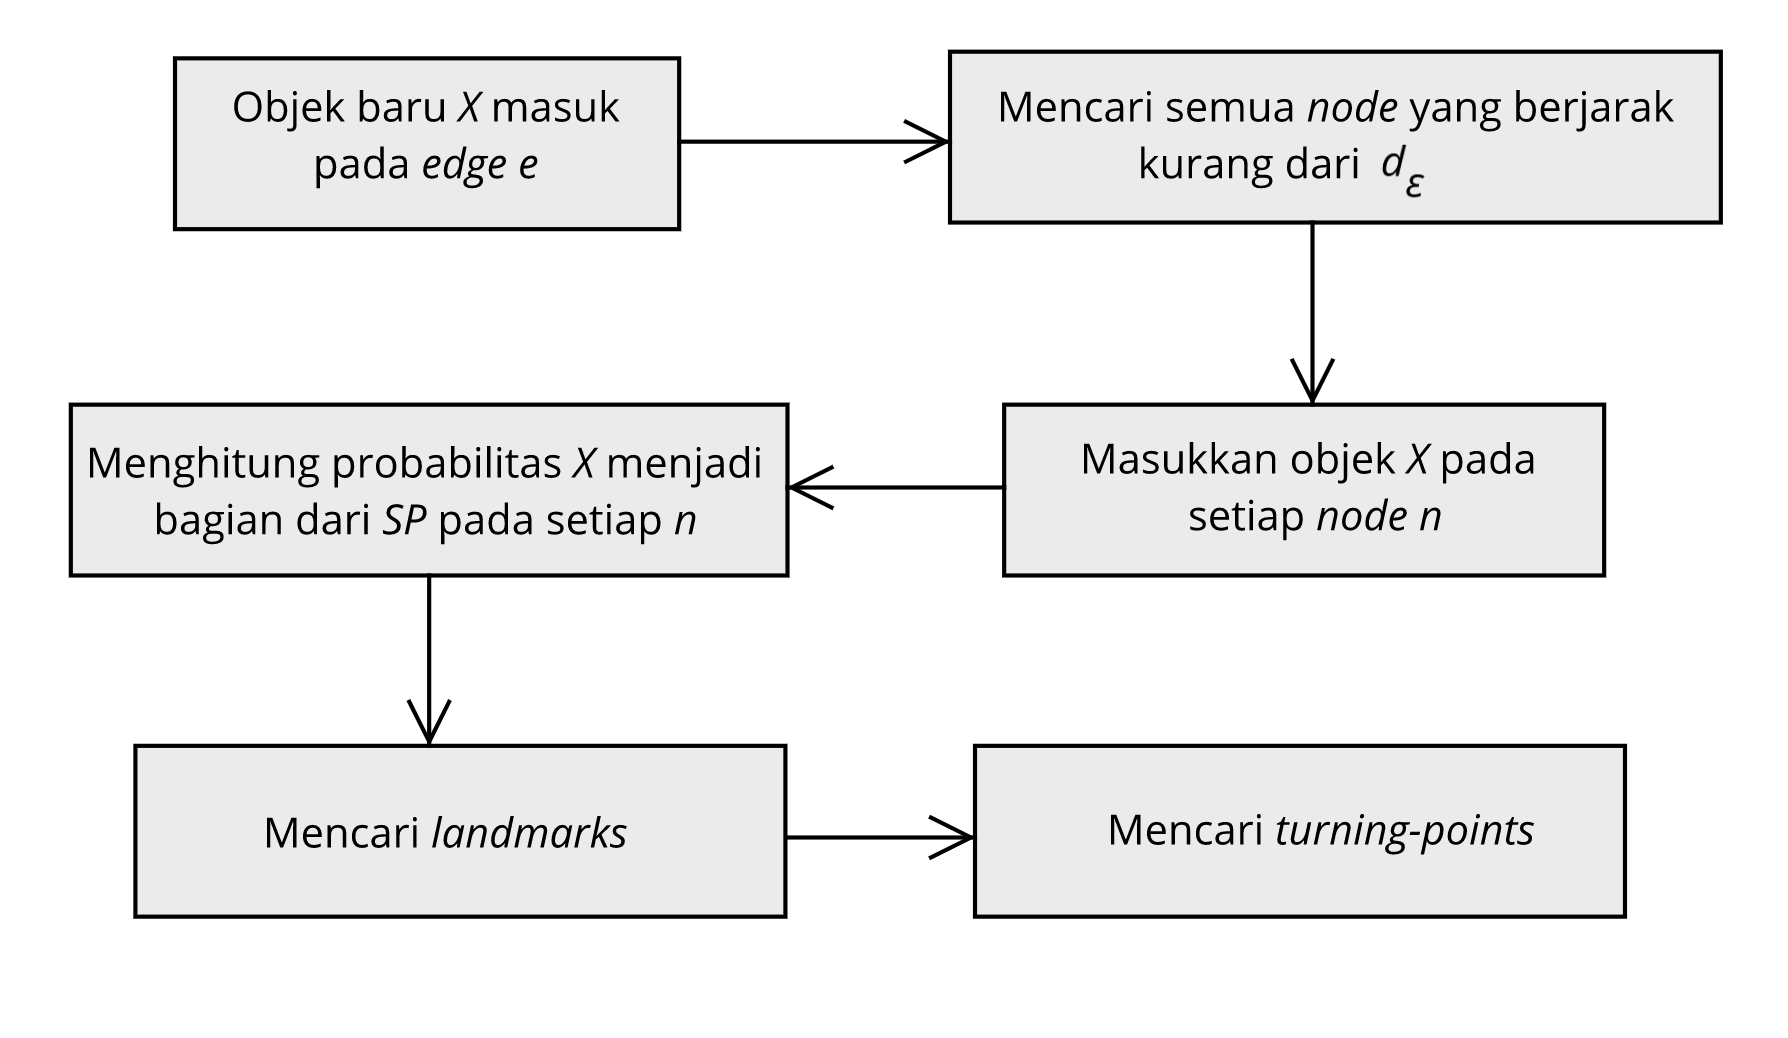
\includegraphics[width=8cm]{imgs/alur.png}
	\caption{Alur pemrosesan}
	\label{fig:alur}
\end{figure}

Perhatikan Gambar \ref{fig:alur} dan Gambar \ref{fig:alur1-2}, saat objek $ X $ yang masuk dari \textit{stream} pada suatu \textit{edge} yang terdapat pada struktur Grid, algoritme BFS mencari semua \textit{node} yang berjarak kurang dari $ d_\varepsilon $ dari objek $ X $, $ d_{X, n} \le d_\varepsilon $.

\begin{figure}[H]
	\centering
	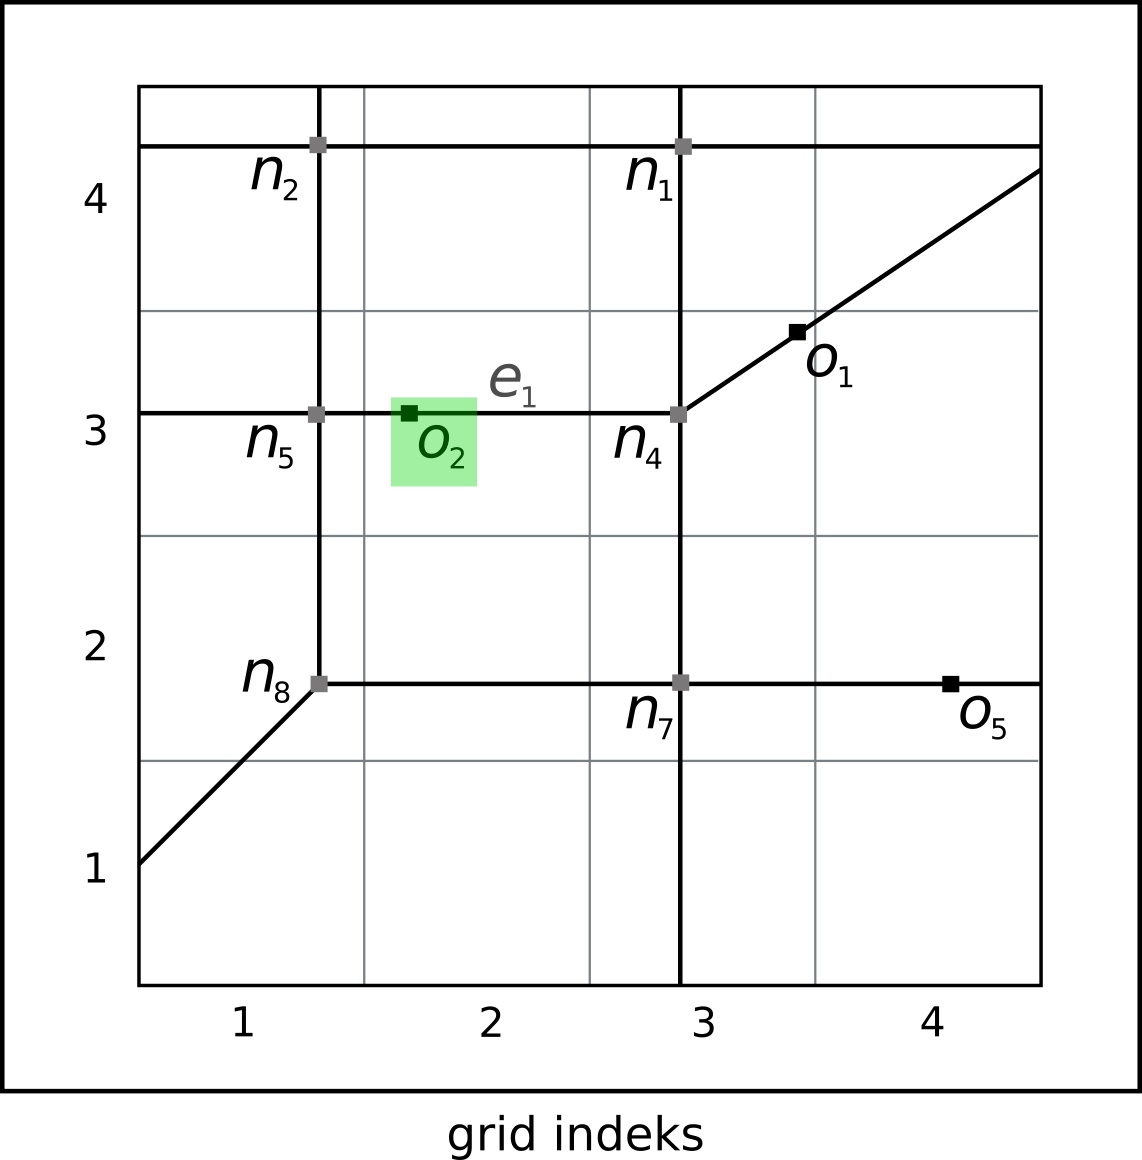
\includegraphics[width=5cm]{imgs/alur/alur1.png}
	\caption{Objek masuk pada grid indeks}
	\label{fig:alur1-2}
\end{figure}

Kemudian objek $ X $ dimasukkan pada struktur data R-Tree yang terdapat pada masing-masing \textit{node} menggunakan algoritme \textit{Insertion}. Setiap objek $ X $ bertahan pada Grid hanya dalam interval waktu yang sama \textit{t}. Jika objek $ X $ sudah kadaluarsa, objek dikeluarkan dari \textit{node} dengan algoritme \textit{Deletion}.

	
	\begin{figure}[H]
		\begin{algorithm}[H]
			\label{algo:insertion}
			\caption{\textit{Insertion}}
			\begin{algorithmic}[1]
				\State \textbf{Input: } uncertain data object $ X $, threshold $ p $
				\For{each object Q overlapped with \textit{PDR(X)}}
				\If{\textit{MBR(Q) is within \textit{DDR(X)}}}
				\State mark \textit{Q} as impossible object
				\Else
				\If{$ \sum_{\textit{q in MBR(Q)$ \cap $DDR(X)}} Pr(q) > (1 - p)$}
				\State mark \textit{Q} as as impossible object
				\Else 
				\State update SkyPr(\textit{Q}) with \textit{X}
				\EndIf
				\EndIf
				\EndFor
				\State compute SkyPr(\textit{X}) with objects overlapped with \textit{PDD(X)}
				\State insert \textit{X} into \textit{SW-Tree}
			\end{algorithmic}
		\end{algorithm}
		\caption{Algoritme \textit{Insertion}}
	\end{figure}

	\begin{figure}[H]
		\begin{algorithm}[H]
			\label{algo:deletion}
			\caption{\textit{Deletion}}
			\begin{algorithmic}[1]
				\State \textbf{Input: }expired uncertain data $ U $, threshold $ p $
				\For{each object \textit{Q} overlapped with \textit{PDR(X) and not marked}}
				\State update SkyPr(\textit{Q}) with removal of \textit{X}
				\EndFor
				\State Remove X from \textit{SW-Tree}
			\end{algorithmic}
		\end{algorithm}
		\caption{Algoritme \textit{Deletion}}
	\end{figure}


Setelah objek masuk pada semua \textit{node} $ n $ $ d_{X, n} \le d_\varepsilon $, proses pencarian \textit{landmark} dilakukan sebagai dasar pencarian \textit{turning-point}. Masukan dari proses pencarian \textit{Landmark} yaitu \textit{GSP}. \textit{GSP} adalah objek-objek yang menjadi $ SP^\varepsilon $ yang terdapat pada $ n_s $ dan $ n_e $ dan objek-objek yang terdapat pada edge $ e $. Terakhir, penentuan \textit{turning-point} dilakukan pada setiap \textit{edge} yang berhubungan dengan $ n $. Hasil akhir dari proses ini adalah \textit{turning-point}.

\begin{figure}
	\centering
	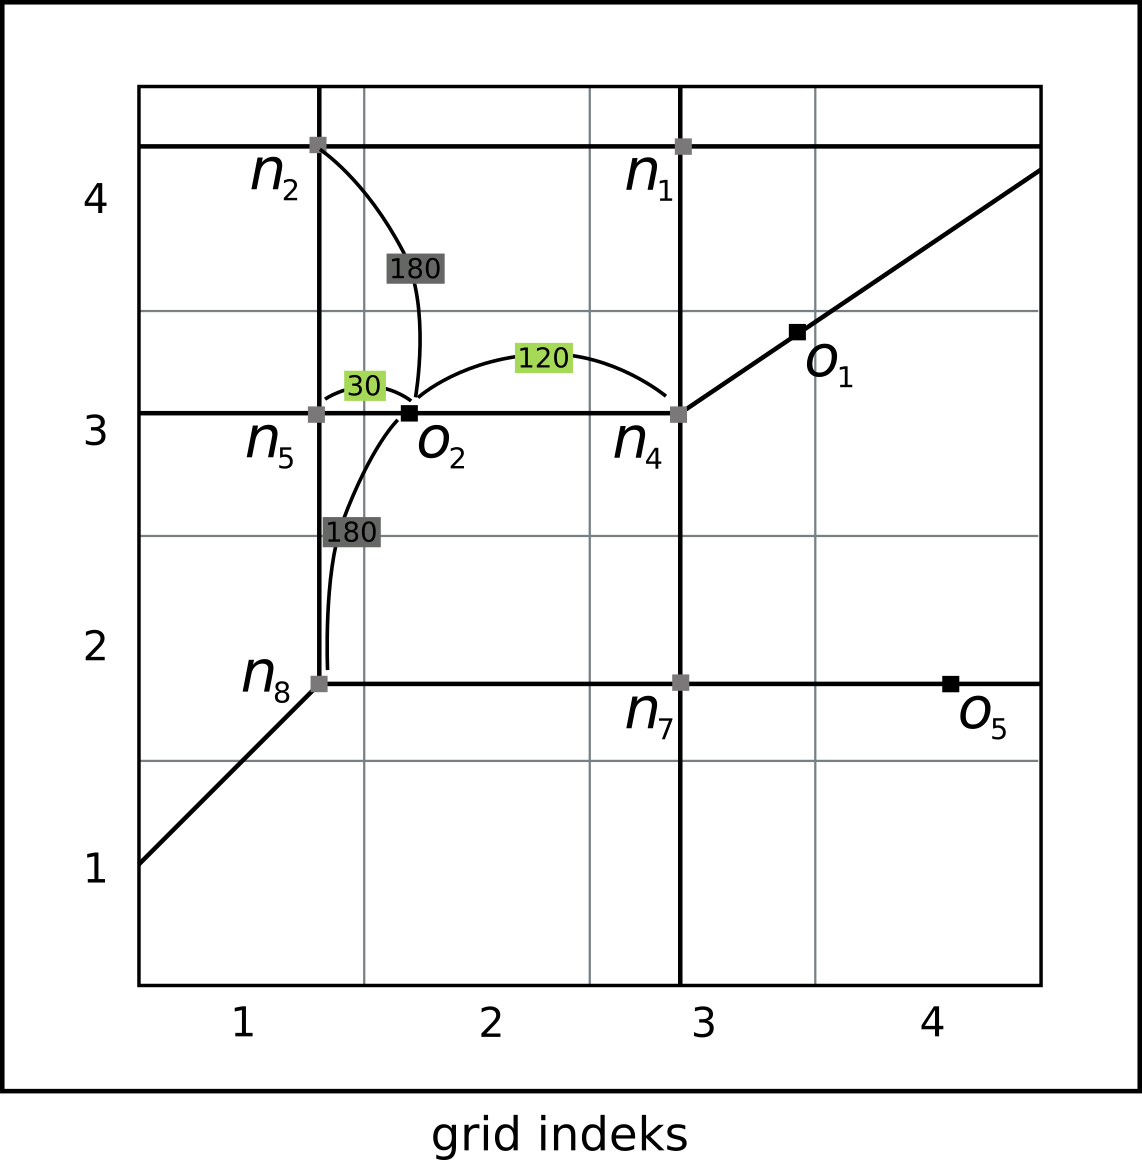
\includegraphics[width=5cm]{imgs/alur/alur3.png}
	\caption{Dengan $ d_\varepsilon $=150, $ o_2 $ hanya masuk pada \textit{node} $ n_4 $ dan $ n_5 $}
	\label{fig:alur3}
\end{figure}

\begin{figure}
	\centering
	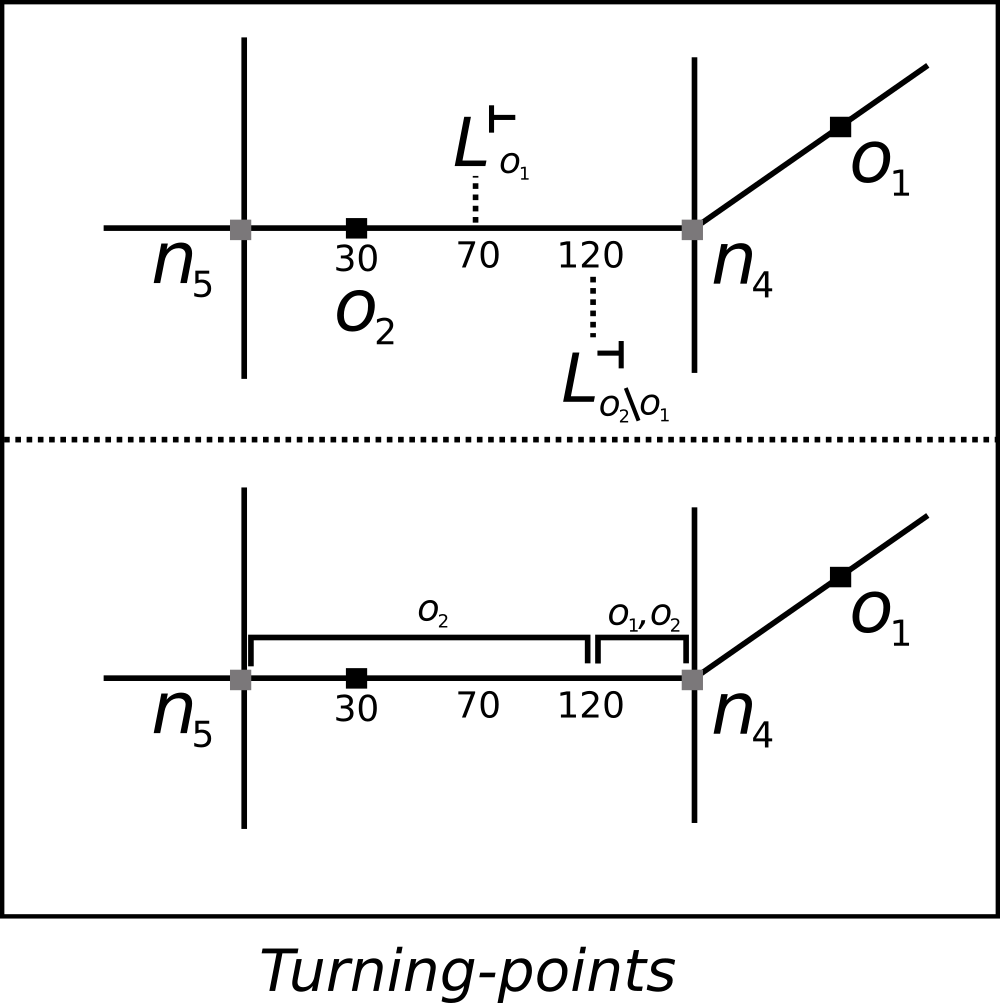
\includegraphics[width=5cm]{imgs/alur/alur6.png}
	\caption{Atas: \textit{landmark} yang didapat dari \textit{edge}. Bawah: \textit{turning-point} didapat dari \textit{landmark}}.
	\label{fig:alur4-5}
\end{figure}

Suatu edge $ e $ pada jaringan jalan raya memiliki dua ujung \textit{node}, yaitu \textit{node} ujung awal $ n_s $ dan \textit{node} ujung akhir $ n_e $. Setiap \textit{node} memiliki objek dan terhubung dengan \textit{edge}. Dari proses  \textit{Skyline} \textit{edge} \textit{e} direpresentasikan dalam bentuk interval beserta \textit{SP} yang terdapat pada masing-masing interval. Antara interval satu dengan interval lain terdapat pergantian objek yang menjadi \textit{SP}. Titik pergantian \textit{SP} ini diistilahkan dengan \textit{turning-point}.

\begin{figure}
	\begin{algorithm}[H]
		\label{compute_turning_point}
		\caption{ComputeTurningPoint}
		\begin{algorithmic}[1]
			\State \textbf{Input: }threshold $ p $, a distance $ d_\varepsilon $, a set \textit{GSP}, an edge \textit{e} connecting two nodes $ n_s $ and $ n_e $
			\State \textbf{Output:} A set of tuples in form of $ < [n_i, n_j], SP^\varepsilon >$ where $ SP^\varepsilon $ is the $ d_\varepsilon-SP $ set between $ [n_i, n_j] $
			\State create an empty queue Q
			\For{object \textit{o} $ \in $ \textit{GSP}}
			\State determine \textit{o}'s landmarks $ L_o^\vdash $ and $ L_o^\dashv $
			\If{$ L_o^\vdash $ is on \textit{e}}
			insert $ L_o^\vdash $ into \textit{Q}
			\EndIf
			\If{$ L_o^\dashv $ is on \textit{e}}
			insert $ L_o^\dashv $ into \textit{Q}
			\EndIf
			\For{object \textit{o'} $ \in (GSP-\{o\}) \cap \sum_{\textit{q in MBR(o')$ \cap $DDR(o)}} Pr(q) > (1 - p) $}
			\State determine \textit{o}'s landmarks $ L_o^\vdash $ or $ L_o^\dashv $
			\If{ $ L_{o \setminus o'}^\vdash $ is on $ e $ and $ L_o^\vdash $ is closer to $ n_s $ than $ L_{o \setminus o'}^\vdash $}
			\State insert $ L_{o \setminus o'}^\vdash $ into \textit{Q}
			\EndIf
			\If{ $ L_{o \setminus o'}^\dashv $ is on $ e $ and $ L_{o \setminus o'}^\dashv $ is closer to $ n_s $ than $ L_{o}^\dashv $}
			\State insert $ L_{o \setminus o'}^\dashv $ into \textit{Q}
			\EndIf
			\EndFor
			\EndFor
			\State sort landmarks in Q in ascending order of their distances to $ n_s $
			
			\State /* determining the result turning points */
			\While{\textit{Q} is not empty}
			\State dequeue $ o.L $
			\Switch{$ o.L $}
			\Case{$ L_o^\vdash $}
			\If{there is no $ L_{o' \setminus o}^\dashv $}
			\State return $ < [n_i, L_o^\vdash], SP^\varepsilon >, n_i =  L_o^\vdash $,
			\State and add \textit{o} into $ SP^\varepsilon $
			\EndIf
			\EndCase
			\Case{$ L_o^\dashv $}
			\If{$ o \in SP^\varepsilon $}
			\State return $ < [n_i, L_o^\dashv], SP^\varepsilon >, n_i =  L_o^\dashv $,
			\State and remove \textit{o} from $ SP^\varepsilon $
			\EndIf
			\EndCase
			\Case{$ L_{o \setminus o'}^\vdash $}
			\If{$ o \in SP^\varepsilon $ and $ o' \in SP^\varepsilon $}
			\State return $ < [n_i, L_{o \setminus o'}^\vdash], SP^\varepsilon >, n_i = L_{o \setminus o'}^\vdash $,
			\State and remove \textit{o'} from $ SP^\varepsilon $
			\EndIf
			\EndCase
			\Otherwise{}
			\If{$ o \in SP^\varepsilon $ and there is no $ L_{o'' \setminus o'}^\dashv \in Q $ }
			\State return $ < [n_i, L_{o \setminus o'}^\dashv], SP^\varepsilon >, $
			\State $ n_i = L_{o \setminus o'}^\dashv, $ and add \textit{o'} into $ SP^\varepsilon $
			\EndIf
			\EndOtherwise
			\EndSwitch
			\EndWhile
		\end{algorithmic}
	\end{algorithm}
	\caption{Algoritme \textit{Compute Turning Point}}
\end{figure}

Algoritma pada Gambar 11 mengilustrasikan penentuan \textit{landmark} pada \textit{edge} $ e $ yang memiliki \textit{node} awal $ n_s $ dan \textit{node} lainnya $ n_e $. Queue $ Q $ dibuat untuk menampung \textit{landmark}. Penentuan landmark ini berdasarkan pada objek-objek yang menjadi anggota dari \textit{GSP}. Setelah mendapatkan semua landmark, \textit{queue} $ Q $ diurutkan berdasarkan jarak terdekat dari \textit{node} $ n_s $.

Setelah semua \textit{landmark} didapatkan, pencarian \textit{turning-point} dilakukan. \textit{Turning-point} ini adalah hasil dari algoritma. \textit{Turning-point} berupa sekumpulan \textit{tuple} yang merepresentasikan interval awal $ n_i $, interval akhir $ n_e $, dan objek-objek yang menjadi $ SP $ pada interval tersebut $ SP^\varepsilon $.

\section{Uji Coba}
Uji coba dilakukan pada jaringan jalan raya California\cite{ontrip} dengan \textit{node} sebanyak 8716 dan \textit{edge} sebanyak 9077. Algoritma diimplementasikan menggunakan bahasa Scala dengan \textit{memory heap} sejumlah 4 GB. Pengujian dilakukan pada komputer dengan \textit{Processor} Intel(R) Core(TM) i3-5010U CPU @ 2.10GHz x 4 dan RAM 6 GB. Pengujian dilakukan untuk mengetahui performa dengan menggunakan waktu komputasi dan untuk mengetahui penggunaan memori pada setiap eksekusi. Uji coba juga dilakukan pada tiga jenis data, yaitu data \textit{independent}, \textit{correlated}, dan \textit{anticorrelated}.

\begin{table}[htbp]
	\caption{Variasi pengujian}
	\begin{center}
		\begin{tabular}{| l | l | l |}
			\hline
			\textbf{Parameter} & \textbf{\textit{Default}} & \textbf {Rentang} \\ \hline
			Jumlah sel grid & $ 256^2 $ & $ 32^2 $, $ 64^2 $, $ 128^2 $, $ 256^2 $, $ 512^2 $ \\ \hline
			Jumlah objek (K) & 5 & 0.1, 1, 5, 10, 20 \\ \hline
			Jumlah \textit{instance} tiap objek & 50 & 10, 50, 100, 200, 400 \\ \hline
			$ d_\varepsilon $ (\%) & 1 & 0.1, 0.5, 1, 2, 3 \\ \hline
			Dimensi data & 2 & 2, 3, 4, 5, 6 \\ \hline
		\end{tabular}
		\label{tab:uji}
	\end{center}
\end{table}

\begin{figure}
	\centering
	\begin{tikzpicture}
	\begin{axis}[
	height=6cm,
	xlabel={Jumlah sel grid},
	ylabel={waktu komputasi (detik/operasi)},
	ymin=0, ymax=1,
	xmin=0, xmax=10,
	xtick={1, 3, 5, 7, 9},
	xticklabels={$ 32^2 $, $ 64^2 $, $ 128^2 $, $ 256^2 $, $ 512^2 $},
	legend pos=north east,
	ymajorgrids=true,
	grid style=dashed,
	]
	
	\addplot[
	color=blue,
	mark=square,
	]
	coordinates {
		(1, 0.198035104400913)(3, 0.19713375528914)(5, 0.214094556217187)(7, 0.177597533827906)(9, 0.213052689078089)
	};
	\addlegendentry{$ CSd_\varepsilon $}
	
	\end{axis}
	\end{tikzpicture}
	\caption{Pengaruh jumlah sel terhadap waktu komputasi tiap operasi dalam satuan detik}\label{fig:uji-g}
\end{figure}

\begin{figure}
	\centering
	\begin{tikzpicture}
	\begin{axis}[
	height=6cm,
	xlabel={Jumlah sel grid},
	ymin=0, ymax=500,
	ylabel={penggunaan memori (MB)},
	xmin=0, xmax=10,
	xtick={1, 3, 5, 7, 9},
	xticklabels={$ 32^2 $, $ 64^2 $, $ 128^2 $, $ 256^2 $, $ 512^2 $},
	legend pos=south east,
	ymajorgrids=true,
	grid style=dashed,
	]
	
	\addplot[
	color=blue,
	mark=square,
	]
	coordinates {
		(1, 205)(3, 245)(5, 222)(7, 209)(9, 214)
	};
	\addlegendentry{$ CSd_\varepsilon $}
	
	\end{axis}
	\end{tikzpicture}
	\caption{Pengaruh jumlah sel grid terhadap penggunaan memori dalam satuan megabita}\label{fig:uji-g-mem}
\end{figure}

Jumlah sel tidak banyak mempengaruhi penggunaan memori dan waktu komputasi. Hal ini dikarenakan adanya \textit{trade-off} antara proses memuat data dengan komputasi. Grid indeks yang memiliki sel sedikit menjadikan data yang dimuat lebih banyak sehingga menjadikan data yang diproses labih banyak. Tetapi di sisi lain, sistem tidak banyak mencari data secara berulang-ulang karena setiap sel sudah mengaver area yang besar. Sedangkan grid indeks yang memiliki sel yang banyak menjadikan proses komputasi lebih efisien karena melibatkan data yang lebih sedikit. Tetapi di sisi lain, sistem harus melakukan pencarian data berulang-ulang karena sedikitnya data yang didapat pada setiap sel.

\begin{figure}
	\centering
	\begin{tikzpicture}
	\begin{axis}[
	width=6cm,
	xlabel={Jumlah objek (k)},
	ymode=log,
	ylabel={waktu komputasi (detik/operasi)},
	xmin=0, xmax=10,
	xtick={1, 3, 5, 7, 9},
	xticklabels={0.1, 1, 5, 10, 20},
	legend pos=south east,
	ymajorgrids=true,
	grid style=dashed,
	]
	
	\addplot[
	color=blue,
	mark=square,
	]
	coordinates {
		(1,0.027)(3, 0.054)(5, 0.24)(7, 0.527)(9, 1.062)
	};
	\addlegendentry{$ CSd_\varepsilon $}
	
	\addplot[
	color=red,
	mark=x,
	]
	coordinates {
		(1,63)(3, 64)(5, 68)(7, 90)(9, 167)
	};
	\addlegendentry{\textit{Naive}}
	
	\end{axis}
	\end{tikzpicture}
	\caption{Pengaruh jumlah objek terhadap waktu komputasi tiap operasi dalam satuan detik}\label{fig:uji-n}
\end{figure}

Ketika jumlah objek bertambah, waktu pemrosesan juga bertambah, hal ini dikarenakan bertambahnya objek yang terdapat pada \textit{node}. Dengan bertambahnya objek pada \textit{node}, algoritme perlu membandingkan dengan objek yang lebih banyak untuk mencari probabilitas masing-masing objek menjadi \textit{SP}.

\begin{figure}
	\centering
	\begin{tikzpicture}
	\begin{axis}[
	width=6cm,
	xlabel={Jumlah objek (k)},
	ymode=log,
	ylabel={penggunaan memori (MB)},
	xmin=0, xmax=10,
	xtick={1, 3, 5, 7, 9},
	xticklabels={0.1, 1, 5, 10, 20},
	legend pos=south east,
	ymajorgrids=true,
	grid style=dashed,
	]
	
	\addplot[
	color=blue,
	mark=square,
	]
	coordinates {
		(1, 16)(3, 41)(5, 328)(7, 367)(9, 375)
	};
	\addlegendentry{$ CSd_\varepsilon $}
	
	\addplot[
	color=red,
	mark=x,
	]
	coordinates {
		(1, 77062)(3, 79292)(5, 78801)(7, 73392)(9, 67442)
	};
	\addlegendentry{\textit{Naive}}
	
	\end{axis}
	\end{tikzpicture}
	\caption{Pengaruh jumlah objek terhadap penggunaan memori dalam satuan megabita}\label{fig:uji-n-mem}
\end{figure}

Terkait penggunaan memori, metode \textit{naive} membutuhkan memori yang sangat banyak karena banyaknya \textit{node} yang perlu diproses menggunakan algoritme \textit{shortest-path}. Sedangkan metode $ CSd_\varepsilon-SQ$ membutuhkan memori yang tidak banyak karena hanya menggunakan data \textit{node} yang diperlukan saja dengan struktur grid.

Jumlah \textit{instance} pada objek mempengaruhi waktu komputasi dan penggunaan memori. Hal ini dikarenakan proses penghitungan probabilitas melibatkan \textit{instances} di objek. Dari sisi memori, banyaknya \textit{instance} membuat sistem harus mengalokasikan memori lebih untuk proses penyimpanan dan komputasi.

\begin{figure}
	\centering
	\begin{tikzpicture}
	\begin{axis}[
	width=6cm,
	xlabel={\textit{instances}},
	ymode=log,
	ylabel={waktu komputasi (detik/operasi)},
	xmin=0, xmax=10,
	xtick={1, 3, 5, 7, 9},
	xticklabels={10, 50, 100, 150, 200},
	legend pos=south east,
	ymajorgrids=true,
	grid style=dashed,
	]
	
	\addplot[
	color=blue,
	mark=square,
	]
	coordinates {
		(1, 0.033)(3, 0.229)(5, 0.979)(7, 3)(9, 5.736)
	};
	\addlegendentry{$ CSd_\varepsilon $}
	
	\addplot[
	color=red,
	mark=x,
	]
	coordinates {
		(1, 67)(3, 70)(5, 74)(7, 133)(9, 132)
	};
	\addlegendentry{\textit{Naive}}
	
	\end{axis}
	\end{tikzpicture}
	\caption{Pengaruh jumlah \textit{instance} terhadap waktu komputasi tiap operasi dalam satuan detik}\label{fig:uji-np}
\end{figure}

Pada metode \textit{naive}, objek perubahan waktu komputasi terlihat ketika jumlah \textit{instance} diatas 100. Hal ini dikarenakan waktu komputasi lebih banyak digunakan untuk penghitungan jarak terpendek dari setiap \textit{node} ke objek, sehingga jumlah \textit{instance} yang sedikit tidak berpengaruh banyak terhadap waktu komputasi.

\begin{figure}
	\centering
	\begin{tikzpicture}
	\begin{axis}[
	width=6cm,
	xlabel={\textit{instances}},
	ymode=log,
	ylabel={penggunaan memori (MB)},
	xmin=0, xmax=10,
	xtick={1, 3, 5, 7, 9},
	xticklabels={10, 50, 100, 150, 200},
	legend pos=south east,
	ymajorgrids=true,
	grid style=dashed,
	]
	
	\addplot[
	color=blue,
	mark=square,
	]
	coordinates {
		(1, 41)(3, 139)(5, 4874)(7, 11213)(9, 32760)
	};
	\addlegendentry{$ CSd_\varepsilon $}
	
	\addplot[
	color=red,
	mark=x,
	]
	coordinates {
		(1, 73772)(3, 81068)(5, 79448)(7, 71448)(9, 58597)
	};
	\addlegendentry{\textit{Naive}}
	
	\end{axis}
	\end{tikzpicture}
	\caption{Pengaruh jumlah \textit{instance} terhadap penggunaan memori dalam satuan megabita}\label{fig:uji-np-mem}
\end{figure}

Jarak $ d_\varepsilon $ sangat mempengaruhi \textit{performance} karena $ d_\varepsilon $ menentukan jarak terjauh \textit{node} yang dapat menyimpan objek baru. Dengan bertambahnya nilai $ d_\varepsilon $, objek dapat menjangkau lebih banyak \textit{node}. Dengan demikian, objek yang ditampung pada \textit{node} menjadi semakin banyak. Dengan semakin banyaknya objek, proses penghiungan probabilitas \textit{skyline} menjadi semakin lama karena harus menghitung banyak objek. Pada $ CSd_\varepsilon-SQ$, semakin besar nilai $ d_\varepsilon $, semakin banyak grid yang diakses sehingga membutuhkan waktu yang lebih banyak. Pada metode \textit{naive}, terdapat perubahan waktu komputasi yang signifikan ketika nilai $ d_\varepsilon $ diatas 1.

\begin{figure}[H]
	\centering
	\begin{tikzpicture}
	\begin{axis}[
	width=6cm,
	xlabel={$ d_\varepsilon $},
	ymode=log,
	ylabel={waktu komputasi (detik/operasi)},
	xmin=0, xmax=10,
	xtick={1, 3, 5, 7, 9},
	xticklabels={0.1, 0.5, 1, 2, 3},
	legend pos=south east,
	ymajorgrids=true,
	grid style=dashed,
	]
	
	\addplot[
	color=blue,
	mark=square,
	]
	coordinates {
		(1, 0.009)(3, 0.052)(5, 0.24)(7, 1.592)(9, 9.667)
	};
	\addlegendentry{$ CSd_\varepsilon $}
	
	\addplot[
	color=red,
	mark=x,
	]
	coordinates {
		(1, 64)(3, 67)(5, 68)(7, 216)(9, 490)
	};
	\addlegendentry{\textit{Naive}}
	
	\end{axis}
	\end{tikzpicture}
	\caption{Pengaruh $ d_\varepsilon $ terhadap waktu komputasi tiap operasi dalam satuan detik}\label{fig:uji-d}
\end{figure}

Penggunaan memori sangat tergantung dari jumlah objek yang diproses. Nilai $ d_\varepsilon $ yang besar menjadikan objek yang diproses semakin banyak karena setiap \textit{node} memiliki jangkauan yang lebih jauh. Banyaknya objek yang diproses menjadikan penggunaan memori semakin besar.

\begin{figure}[H]
	\centering
	\begin{tikzpicture}
	\begin{axis}[
	width=6cm,
	xlabel={$ d_\varepsilon $},
	ymode=log,
	ylabel={penggunaan memori (MB)},
	xmin=0, xmax=10,
	xtick={1, 3, 5, 7, 9},
	xticklabels={0.1, 0.5, 1, 2, 3},
	legend pos=south east,
	ymajorgrids=true,
	grid style=dashed,
	]
	
	\addplot[
	color=blue,
	mark=square,
	]
	coordinates {
		(1, 12)(3, 122.7)(5, 328)(7, 5932)(9, 37507)
	};
	\addlegendentry{$ CSd_\varepsilon $}
	
	\addplot[
	color=red,
	mark=x,
	]
	coordinates {
		(1, 74387)(3, 72904)(5, 78801)(7, 126323)(9, 230699)
	};
	\addlegendentry{\textit{Naive}}
	
	\end{axis}
	\end{tikzpicture}
	\caption{Pengaruh $ d_\varepsilon $ terhadap penggunaan memori dalam satuan megabita}\label{fig:uji-d-mem}
\end{figure}

\section{Kesimpulan}
Pada bab ini dijelaskan mengenai kesimpulan dan saran dari hasil uji coba yang telah dilakukan.

Dari proses desain hingga uji coba, dapat diambil beberapa hasil sebagai berikut:

\begin{enumerate}
	\item Artikel ini mengusulkan struktur data grid indeks dan metode $ CSd_\varepsilon $ untuk pengolahan \textit{skyline query} pada \textit{uncertain data streaming} oleh titik bergerak dan objek tidak bergerak. Struktur data grid indeks memecah struktur data graf tradisional menjadi sel-sel yang berisi \textit{node}, \textit{edge}, dan objek. Penyimpanan objek dalam bentuk \textit{SW-Tree} pada setiap \textit{node} membuat proses komputasi lebih cepat.
	
	\item Biaya komputasi pada metode $ CSd_\varepsilon $ jauh lebih baik dibandingkan metode \textit{naive} dari sisi waktu komputasi dan penggunaan memori. Komputasi metode $ CSd_\varepsilon $ lebih cepat 600 kali dibandingkan metode \textit{naive}. Dari sisi penggunaan memori, metode $ CSd_\varepsilon $ lebih hemat 1500 kali dibandingkan metode \textit{naive}.
\end{enumerate}

Berikut beberapa saran terkait pengembangan struktur data dan algoritma lebih lanjut:

\begin{enumerate}
	\item Pendefinisian jarak $ d_\varepsilon $ dapat dilakukan secara dinamis. Apabila pencarian objek dengan jarak $ d_\varepsilon $ tidak menemukan hasil yang diminta, jarak $ d_\varepsilon $ dapat diperbesar secara dinamis hingga mendapatkan hasil yang sesuai.
	\item Pengembangan algoitma untuk memproses objek \textit{uncertain} yang dapat bergerak secara dinamis.
	\item Pada algoritme ini proses pembaruan \textit{instance} dari \textit{uncertain} objek dilakukan dengan menghapus dan menambahkan objek baru. Hal ini tentunya tidak efisien. Diperlukan algoritme pembaruan objek agar lebih efisien dalam hal waktu komputasi dan penggunaan memori.
\end{enumerate}

\begin{thebibliography}{00}

\bibitem{continuousdbased} 
Yuan-Ko Huang, Chia-heng Chang, Chiang Lee, "Continuous distance-based skyline queries in road networks", \textit{Information Systems}, vol 37, no 7, pp. 611-633, 2012.

\bibitem{effectiveprob}
Liu, Chuan-Ming, Tang, Syuan-Wei, "An effective probabilistic skyline query process on uncetain data streams", in \textit{The 6th International Conference on Emerging Ubiquitous Systems and Persuasive Networks}, Londok, UK, 2016.

\bibitem{contmonit}
Xiaofeng Ding, Xiang Lian, Lei Chan, Hai Jin, "Continuous monitoring of skylines over uncertain data streams", \textit{Information Systems}, vol 184, no 1, pp. 196-214, 2012.

\bibitem{surveyuncertaindata}
Yijie Wang, Xiaoyong Li, Yuan Wang, "A Survey of queries over uncertain data", \textit{Knowledge and Information Systems}, vol 37, no 3, pp 485-530, 2013.

\bibitem{managinguncertain}
Wenjie Zhang, Xuemin Lin, Jian Pei, Ying Zhang, "Managing Uncertain Data: Probabilistic Approaches", \textit{Web-Age Information Management}, 2008

\bibitem{ontrip}
Feifei Li, Dihan Cheng, Marios Hadjieleftheriou, George Kollios, Shang-Hua Teng, "On Trip Planning Queries in Spatial Databases", \textit{Advances in Spatial and Temporal Databases}, vol 3633, pp 273-290, 2005

\end{thebibliography}

\end{document}
